\section{Attachements}
\subsection{Vorbereitung}
\subsubsection{Attachement A}


\subsubsection{Attachement B}


\subsubsection{Attachement D}


\subsubsection{Attachement E}


\subsection{Lowpass filter}
\subsubsection{Attachement F}

	\begin{figure}[h]
		\centering
		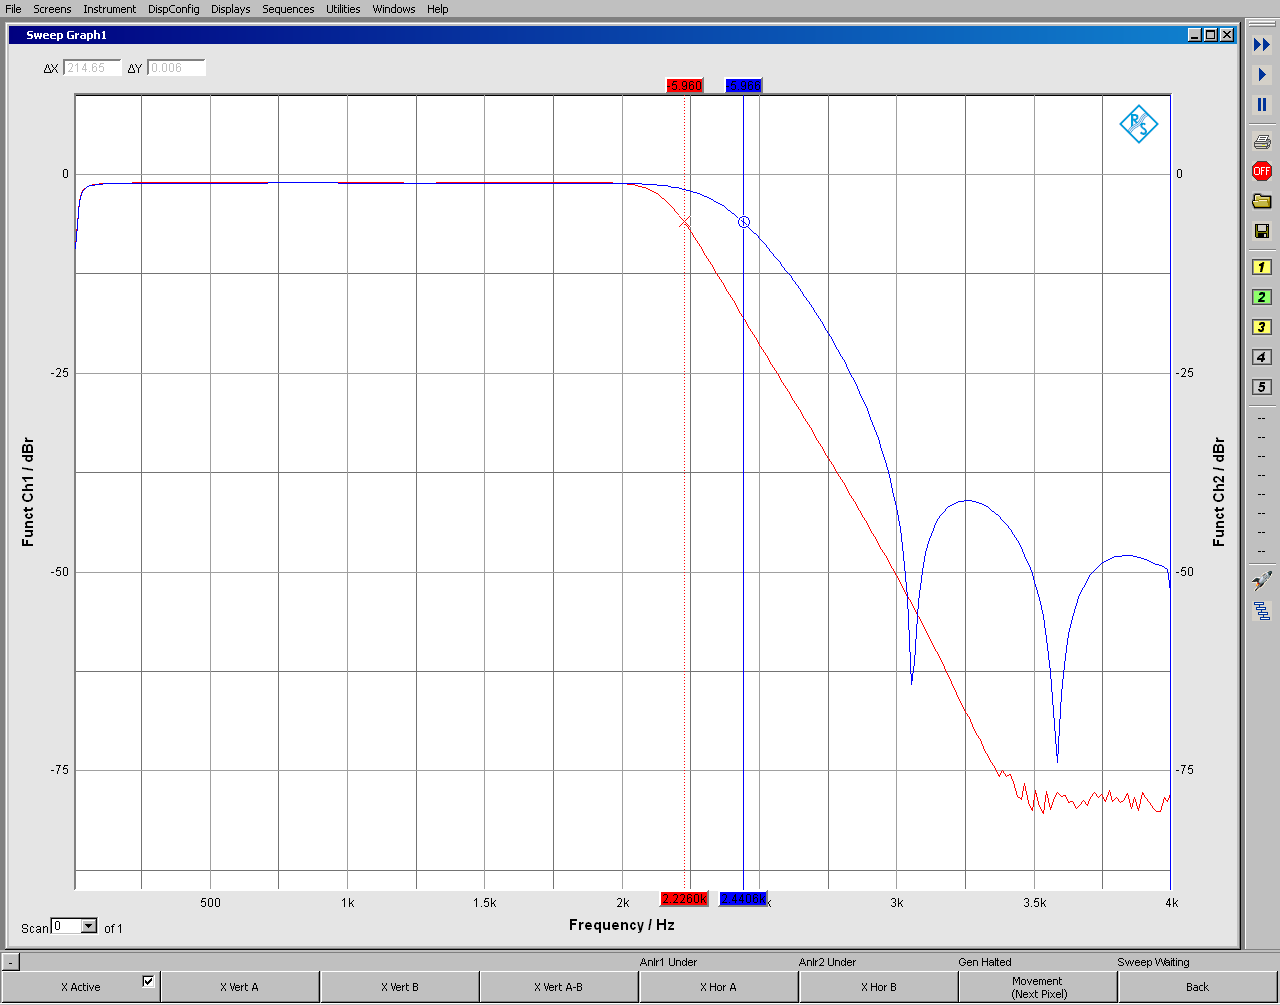
\includegraphics[width=0.8\linewidth]{Bilder/EllipCheby}
		\caption{Blau: Elliptisches IIR TP-Filter | Rot: Chebychev IIR TP-Filter}
		\label{fig:EllipCheby}
	\end{figure}
	
\noindent Der linke Ausgang lieferte das mit einem elliptischen TP-Filter gefilterte Eingangssignal (blau), der rechte Ausgang lieferte das mit einem Chebychev-TP-Filter gefilterte Eingangssignal (rot). Ein Frequenzsweep von 0 .. 4kHz wurde für die Messungen durchgeführt. Die Filterrealisierung geschah jeweils über k kaskadierter Biquads zweiter Ordnung. Für das elliptische Filter war k = 2, für Chebychev war k = 3.

\subsubsection{Attachement G}


\subsection{Hochpass - Tiefpass - Weichenfilter}


\subsection{Modifiziertes elliptisches Tiefpassfilter}
\subsubsection{Attachement H}


\subsubsection{Attachement J}


\subsubsection{Attachement K}

	\begin{figure}[h]
		\centering
		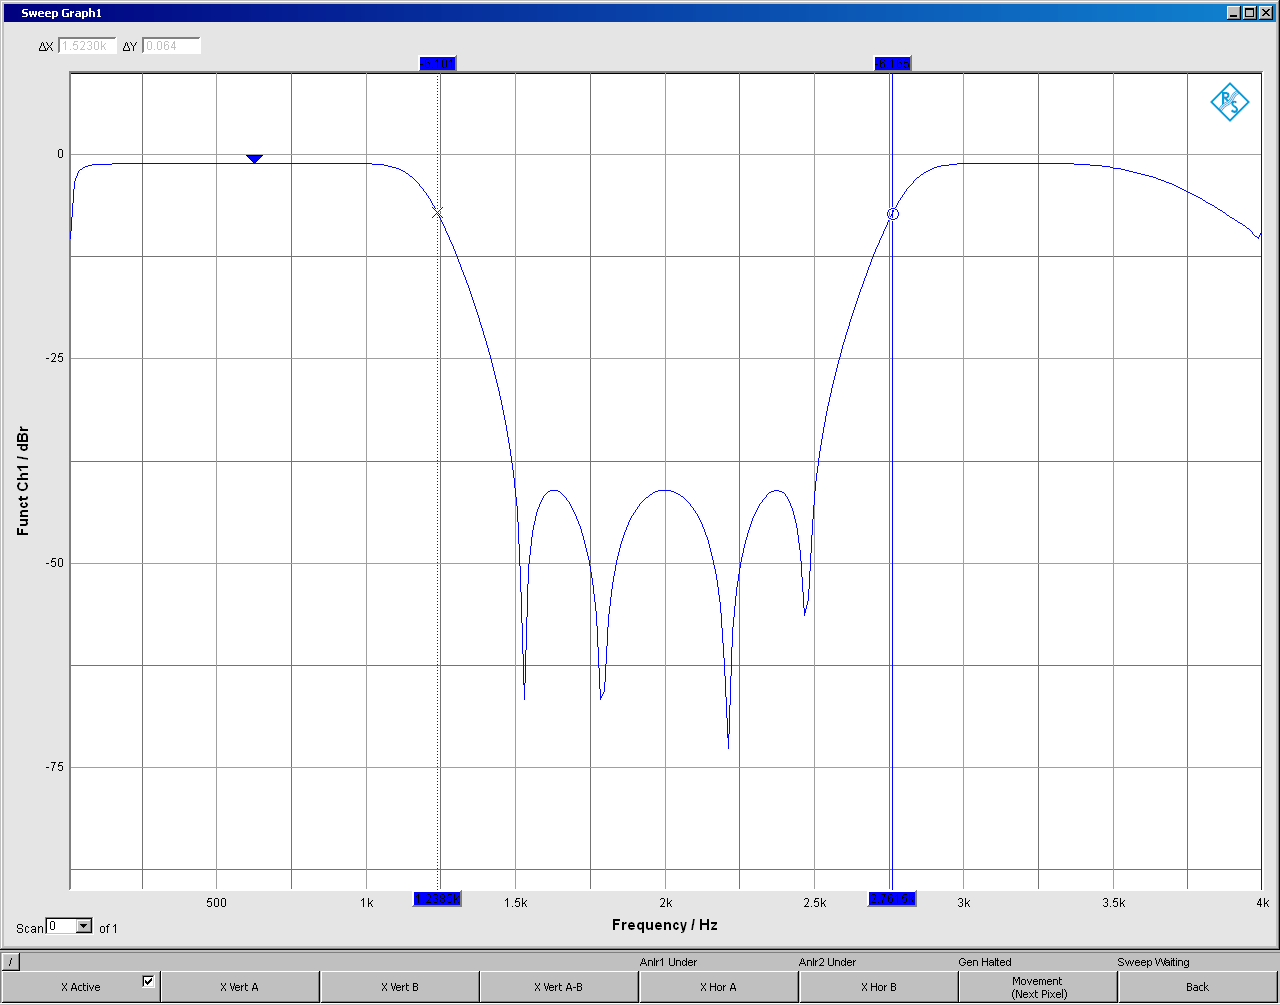
\includegraphics[width=0.7\linewidth]{Bilder/ellip2T}
		\caption{Frequenzgang modifiziertes Tiefpassfilter $|T| \rightarrow |2T|$}
		\label{fig:ellip2T}
	\end{figure}
